\chapter[Hybrid Quantum-Classical Algorithms]{Hybrid Quantum-Classical\\Algorithms} \label{chap:hybrid-quantum-classical-algorithms}
At the end of the previous chapter, two important quantum algorithms were reviewed: the \gls{qft} and Grover's algorithm.
These quantum algorithms and the family of algorithms built on them require large-scale quantum computers with low error rates and high coherence.
The \gls{nisq} devices that are being built now and in the near future will not be able to run these algorithms.
To this end, \acrfullpl{hqca} that utilize both classical and quantum resources are being researched and developed.
This chapter will first introduce the basic concepts of an important family of \glspl{hqca} followed by a review of well-known and promising \glspl{hqca}.

\section{Variational Hybrid Quantum-Classical Algorithms}
\Acrlongpl{hqca} account for the limited number of qubits, limited connectivity of qubits, and limited coherence times of \gls{nisq} devices.
These algorithms often make use of the variational method which consists of preparing an initial trial state $\ket{\psi(\vec{\theta})}$ parameterized by real-valued parameters $\vec{\theta}$, and finding the parameters for which the expectation value of some observable is the lowest.
This family of \glspl{hqca} is sometimes also referred to as variational quantum algorithm, as it uses the variational method of quantum mechanics.
The rest of this chapter will be focused on variational \glspl{hqca}.

The general structure of a variational \gls{hqca} is shown in \Cref{fig:vqa-general-structure}.
While the specific implementation differs between algorithms, they all share some basic elements.
First, a cost function $C$ which encodes the solution to the problem needs to be defined.
Second, an ansatz needs to be chosen.
The ansatz defines the operations of the quantum circuit which are parameterized by the trainable parameters $\vec{\theta}$.
\begin{figure}[ht]
    \centering
    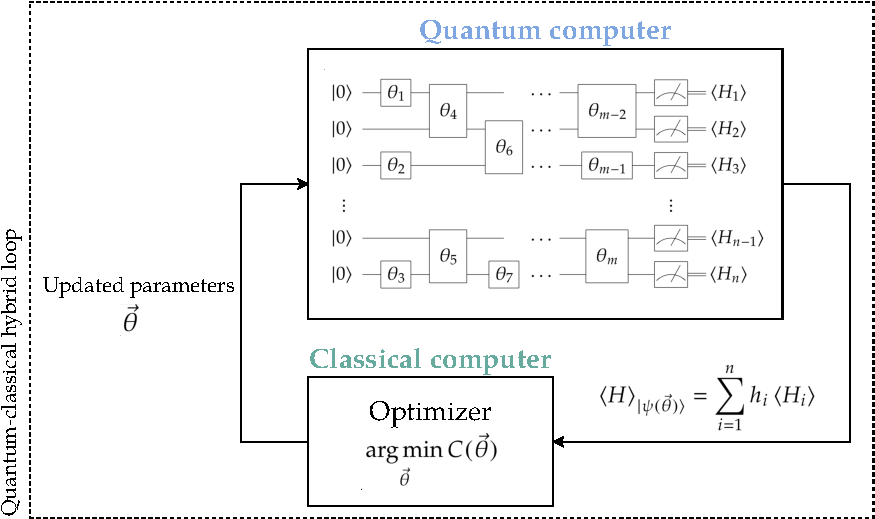
\includegraphics[width=1\linewidth]{figures/vqa-general-structure.pdf}
    \caption[The general structure of a variational \acrshort{hqca}.]{The general structure of a variational \gls{hqca}. A parameterized quantum state $\ket{\psi(\vec{\theta})}$ is prepared through a set of parameterized quantum gates $U_L(\vec{\theta}_L) \ldots U_2(\vec{\theta}_2)U_1(\vec{\theta}_1)$. These parameters classically optimized according to a cost function $C(\vec{\theta})$. This quantum-classical loop is repeated until convergence.}
    \label{fig:vqa-general-structure}
\end{figure}
The parameters $\vec{\theta}$ are then trained in a quantum-classical loop to solve the optimization problem
\begin{equation}
\argmin_{\vec{\theta}} C(\vec{\theta}).
\end{equation}

\subsection{Cost Function}
In general, the cost function has the form
\begin{equation}
C(\vec{\theta}) = \sum_k f_k\left(\bra{0^n}U(\vec{\theta})^\dagger H_k U(\vec{\theta})\ket{0^n}\right),
\end{equation}
where $f_k$ is a function encoding the problem at hand, $U(\vec{\theta})$ is the parameterized ansatz, $H_k$ is an observable, and $n$ is the number of qubits.
A key point of variational \glspl{hqca} is that a quantum computer is used to estimate $C(\vec{\theta})$ while using a classical computer to optimize the parameters $\vec{\theta}$.
Furthermore, the cost function $C(\vec{\theta})$ should be efficient to estimate by performing measurements on a quantum computer.
For the variational \gls{hqca} to have a quantum advantage, the cost should also not be efficiently computable with a classical computer.

\subsection{Ansatze}
To keep the algorithm realizable on \gls{nisq} devices, it is important to keep the parameterized quantum circuit relatively shallow in depth.

\subsection{Optimizers}


\section{Variational Quantum Eigensolver}

\section{Quantum Approximate Optimization Algorithm}